\documentclass[12pt, a4paper, oneside]{Thesis} % Paper size, default font size and one-sided paper
\usepackage{wrapfig}
\usepackage{lscape}
\usepackage{rotating}
\usepackage{graphicx}
\usepackage{caption}
\usepackage{amsmath}
\usepackage{tabularray}
\usepackage{booktabs}
\usepackage{multirow}
\usepackage{tcolorbox}
\usepackage{graphicx} 
\usepackage{mdframed}
\usepackage{colortbl}
\usepackage{enumitem}
\usepackage{tikz}
\usetikzlibrary{shapes.geometric, arrows, positioning, fit, backgrounds, calc, shadows, decorations.pathmorphing}
\usepackage{tabularx} % Add this line in the preamble


\usepackage{lineno,hyperref}
\modulolinenumbers[5]


\usepackage{amssymb}
\usepackage{graphicx}
\usepackage{array}
\usepackage{float}
\usepackage{placeins}
\usepackage{stackengine}
\usepackage{url}
\usepackage{numprint}
\usepackage{caption}
\usepackage{hyperref}
\usepackage{booktabs}
\usepackage{siunitx}
% \usepackage[showframe=false]{geometry}
\usepackage{subfigure}
\usepackage{listings}
\usepackage{xcolor}

% \documentclass{article}

%New colors defined below
\definecolor{codegreen}{rgb}{0,0.6,0}
\definecolor{codegray}{rgb}{0.5,0.5,0.5}
\definecolor{codepurple}{rgb}{0.58,0,0.82}
\definecolor{backcolour}{rgb}{0.95,0.95,0.92}

%Code listing style named "mystyle"
\lstdefinestyle{mystyle}{
  backgroundcolor=\color{backcolour},   commentstyle=\color{codegreen},
  keywordstyle=\color{magenta},
  numberstyle=\tiny\color{codegray},
  stringstyle=\color{codepurple},
  basicstyle=\ttfamily\footnotesize,
  breakatwhitespace=false,
  breaklines=true,
  captionpos=b,
  keepspaces=true,
  numbers=left,
  numbersep=5pt,
  showspaces=false,
  showstringspaces=false,
  showtabs=false,
  tabsize=2
}

%"mystyle" code listing set
\lstset{style=mystyle}


\nprounddigits{3}
\newcolumntype{P}[1]{>{\centering\arraybackslash}p{#1}}
\newcolumntype{M}[1]{>{\centering\arraybackslash}m{#1}}

\setstackEOL{\#}
\setstackgap{L}{12pt}


%\usepackage{subcaption} %incompatible with subfig
\graphicspath{{Pictures/}} % Specifies the directory where pictures are stored
\usepackage{natbib} % Use the natbib reference package - read up on this to edit the reference style; if you want text (e.g. Smith et al., 2012) for the in-text references (instead of numbers), remove 'numbers' v

\hypersetup{urlcolor=black, colorlinks=false} % Colors hyperlinks in blue - change to black if annoyingv`

\thesistitle{SmokeCtrl: AI-Driven Mobile App for Tobacco Cessation Using Agentic Dialogues}
\supervisor{Professor Jayanta Mukhopadhyay}
\degree{Master of Technology}
\degreemajor{Computer Science and Engineering}
\authors{Hardik Pravin Soni}
\rollno{20CS30023}
\university{Indian Institute of Technology Kharagpur}
\department{Department of Computer Science and Engineering}
\unisite{http://www.iitkgp.ac.in}
\depsite{https://cse.iitkgp.ac.in/}
\placeshrt{Kharagpur}
\placelng{Kharagpur - 721302, India}
\datesub{April 22, 2025}
\datesig{April 22, 2025}
\semsub{Spring Semester, 2024-25}
\keywords{Steel Structure}
\coursecd{Project-IV (CS57004) }

\usepackage{listings}
\lstset{
  basicstyle=\scriptsize\ttfamily,
  breaklines=true,
  frame=none,
  backgroundcolor=\color{gray!5},
  columns=fullflexible
}

\title{\ttitle} % Defines the thesis title - don't touch this
\begin{document}
%\makeatletter
%\renewcommand*{\NAT@nmfmt}[1]{\textsc{#1}}
%\makeatother

% prints author names as small caps


\frontmatter % Use roman page numbering style (i, ii, iii, iv...) for the pre-content pages

\setstretch{1} % Line spacing of 1.6 (double line spacing)

% Define the page headers using the FancyHdr package and set up for one-sided printing
\fancyhead{} % Clears all page headers and footers
\rhead{\thepage} % Sets the right side header to show the page number
\lhead{} % Clears the left side page header

%\pagestyle{fancy} % Finally, use the "fancy" page style to implement the FancyHdr headers

\newcommand{\HRule}{\rule{\linewidth}{0.5mm}} % New command to make the lines in the title page

% PDF meta-data
\hypersetup{pdftitle={\ttitle}}
\hypersetup{pdfsubject=\subjectname}
\hypersetup{pdfauthor=\authornames}
\hypersetup{pdfkeywords=\keywordnames}

%----------------------------------------------------------------------------------------
%	TITLE PAGE
%----------------------------------------------------------------------------------------
\maketitle
%\titlepg % Add a gap in the Contents, for aesthetics

\clearpage % Start a new page

%----------------------------------------------------------------------------------------
%	DECLARATION PAGE
%	Your institution may give you a different text to place here
%----------------------------------------------------------------------------------------


\Declaration% Add a gap in the Contents, for aesthetics


%----------------------------------------------------------------------------------------
%	CERTIFICATE PAGE
%----------------------------------------------------------------------------------------

\addtotoc{Certificate} % Add the "Abstract" page entry to the Contents

\certificate{\addtocontents{toc}{}} % Add a gap in the Contents, for aesthetics

\clearpage % Start a new page

%----------------------------------------------------------------------------------------
%	ABSTRACT PAGE
%----------------------------------------------------------------------------------------

\addtotoc{Abstract} % Add the "Abstract" page entry to the Contents

\abstract{\addtocontents{toc}{} % Add a gap in the Contents, for aesthetics
\textbf{SmokeCtrl: A Flutter-based mobile app leveraging Llama 3.2 and agentic-based conversation generation to support and guide tobacco cessation for a healthier, smoke-free life.}

\textbf{SmokeCtrl} is a mobile application developed using \textbf{Flutter}, designed specifically to assist patients in overcoming \textbf{tobacco addiction}. By leveraging the capabilities of \textbf{large language models (LLMs)}, SmokeCtrl provides \textit{intelligent} and \textit{tailored} responses to users' medical queries, supporting their journey towards cessation. The application features:

\begin{itemize}
    \item A \textbf{simple, dynamic, and user-friendly UI} for easy navigation, offering \textbf{login} and \textbf{sign-up} functionalities.
    \item Back-end integration with \textbf{Spring} to manage user authentication and database operations.
    \item \textbf{Llama 3.2-based model inference}, offering interactive and responsive dialogue for users by generating relevant responses to prompts.
    \item \textbf{Retrieval-Augmented Generation (RAG)} setup using \textbf{LangChain}, with a \textit{Chroma database} to support \textit{context-aware} response generation.
    \item Fine-tuning of \textbf{Llama 3.2} using \textbf{Quantized Low-Rank Adaptation (qLoRA)} to optimize performance specifically for conversational and retrieval tasks.
    \item A novel \textbf{doc2conv} agentic-based library that enables \textit{automated generation} of high-quality synthetic conversations for model fine-tuning.
    \item Integration with multiple \textbf{LLM providers} (OpenAI, Google Gemini, Anthropic Claude, Groq, Ollama) for flexible and robust conversation generation.
    \item \textbf{Chain-of-thought reasoning} capabilities that enhance the transparency and quality of generated healthcare advice.
\end{itemize}

Beyond assisting individual users, SmokeCtrl contributes to \textbf{societal well-being} by:

\begin{enumerate}
    \item Encouraging \textbf{public health awareness} about tobacco’s adverse effects, reaching a broad audience through \textbf{mobile accessibility}.
    \item Reducing \textbf{healthcare costs} by promoting early interventions and preventive measures in tobacco cessation.
    \item Supporting \textbf{healthcare providers} with valuable insights
    into patient progress, facilitating better-targeted support.
    \item Enhancing \textbf{mental and emotional well-being} by providing round-the-clock access to resources and personalized motivation.
    \item Strengthening \textbf{community health} by promoting a culture of wellness and offering a tool for family and friends to support users in their cessation journey.
    \item Advancing \textbf{AI research in healthcare} through the development of agentic systems that can generate high-quality, domain-specific training data.
\end{enumerate}

\textbf{Keywords}: Tobacco cessation, Flutter application, large language model, retrieval-augmented generation, Quantized qLoRA, agentic systems, synthetic data generation

}

\clearpage % Start a new page



%----------------------------------------------------------------------------------------
%	ACKNOWLEDGEMENTS
%----------------------------------------------------------------------------------------

\setstretch{1.0} % Reset the line-spacing to 1.3 for body text (if it has changed)

\acknowledgements{\addtocontents{toc}{}%\vspace{1em}} % Add a gap in the Contents, for aesthetics

I express my sincere gratitude to my supervisor, Professor Jayanta Mukhopadhyay, for granting me the opportunity to work under his mentorship. Throughout my M.Tech project, he provided insightful guidance and constructive feedback. He was consistently supportive and understanding.

I am grateful for the chance to have worked on this project and to have learned from the people I have met along the way. This project has been challenging but rewarding, and I am proud of what I have achieved. I would also like to extend my warmest gratitude to my family and friends at IIT Kharagpur for their unwavering support and motivation throughout my journey.
}
\clearpage % Start a new page

%----------------------------------------------------------------------------------------
%	LIST OF CONTENTS/FIGURES/TABLES PAGES
%----------------------------------------------------------------------------------------

\pagestyle{fancy} % The page style headers have been "empty" all this time, now use the "fancy" headers as defined before to bring them back

\lhead{\emph{Contents}} % Set the left side page header to "Contents"
\tableofcontents % Write out the Table of Contents

\lhead{\emph{List of Figures}} % Set the left side page header to "List of Figures"
\listoffigures % Write out the List of Figures

\lhead{\emph{List of Tables}} % Set the left side page header to "List of Tables"
\listoftables % Write out the List of Tables

%----------------------------------------------------------------------------------------
%	ABBREVIATIONS
%----------------------------------------------------------------------------------------

\clearpage % Start a new page

\setstretch{1.5} % Set the line spacing to 1.5, this makes the following tables easier to read

\lhead{\emph{Abbreviations}} % Set the left side page header to "Abbreviations"
\listofsymbols{ll} % Include a list of Abbreviations (a table of two columns)
{

\textbf{LLM} & \textbf{L}arge \textbf{L}anguage \textbf{M}odel \\
\textbf{NLP} & \textbf{N}atural \textbf{L}anguage \textbf{P}rocessing \\
\textbf{mHealth} & \textbf{M}obile \textbf{H}ealth \\
\textbf{RAG} & \textbf{R}etrieval-\textbf{A}ugmented \textbf{G}eneration \\
\textbf{qLoRA} & \textbf{Q}uantized \textbf{L}ow-\textbf{R}ank \textbf{A}daptation \\
\textbf{UI} & \textbf{U}ser \textbf{I}nterface \\
\textbf{API} & \textbf{A}pplication \textbf{P}rogramming \textbf{I}nterface \\
\textbf{JWT} & \textbf{J}SON \textbf{W}eb \textbf{T}oken (used for authentication) \\
\textbf{CRUD} & \textbf{C}reate, \textbf{R}ead, \textbf{U}pdate, \textbf{D}elete (basic database operations) \\
\textbf{GPU} & \textbf{G}raphics \textbf{P}rocessing \textbf{U}nit \\
\textbf{ML} & \textbf{M}achine \textbf{L}earning \\
\textbf{AI} & \textbf{A}rtificial \textbf{I}ntelligence \\
\textbf{SSL} & \textbf{S}ecure \textbf{S}ockets \textbf{L}ayer (for secure data transmission) \\
\textbf{HTTP} & \textbf{H}ypertext \textbf{T}ransfer \textbf{P}rotocol \\
\textbf{SDK} & \textbf{S}oftware \textbf{D}evelopment \textbf{K}it \\
\textbf{UX} & \textbf{U}ser \textbf{E}xperience \\
\textbf{DB} & \textbf{D}atabase \\
\textbf{OAuth} & \textbf{O}pen \textbf{A}uthorization (often used for user authentication) \\
\textbf{REST} & \textbf{R}epresentational \textbf{S}tate \textbf{T}ransfer (API architectural style) \\
\textbf{CoT} & \textbf{C}hain-\textbf{o}f-\textbf{T}hought (reasoning process in LLMs) \\
\textbf{doc2conv} & \textbf{Doc}ument \textbf{to} \textbf{Conv}ersation (agentic library for synthetic data generation) \\
\textbf{SFT} & \textbf{S}upervised \textbf{F}ine-\textbf{T}uning (method for training LLMs on specific tasks) \\
}

%----------------------------------------------------------------------------------------
%	PHYSICAL CONSTANTS/OTHER DEFINITIONS
%----------------------------------------------------------------------------------------
%
%\clearpage % Start a new page
%
%\lhead{\emph{Physical Constants}} % Set the left side page header to "Physical Constants"
%
%\listofconstants{lrcl} % Include a list of Physical Constants (a four column table)
%{
%Speed of Light & $c$ & $=$ & $2.997\ 924\ 58\times10^{8}\ \mbox{ms}^{-\mbox{s}}$ (exact)\\
%% Constant Name & Symbol & = & Constant Value (with units) \\
%}

%----------------------------------------------------------------------------------------
%	SYMBOLS
%----------------------------------------------------------------------------------------

\clearpage % Start a new page

% \lhead{\emph{Symbols}} % Set the left side page header to "Symbols"

% \listofnomenclature{lll} % Include a list of Symbols (a two column table)
% {
% $\psi$ & Eigen Vector & \\
% $||\?\rangle$ & Quantum Bit & \\
% $H$ & Hadamard Gate & \\
% $X$ & Pauli X Gate & \\
% $Y$ & Pauli Y Gate & \\
% $Z$ & Pauli Z Gate & \\
% $SWAP$ & Swap Quantum Gate & \\
% $CNOT$ & Controlled-NOT Gate & \\
% $CP(\lambda)$ & Controlled Phase Gate & \\
% $\mathbb{C}$ & Complex Number & \\
% $\oplus$ & Tensor Product & \\
% $\theta$ & Phase & \\
% $CROT_k$ & Two-qubit controlled rotation in Block-diagonal Form & \\
% }
%----------------------------------------------------------------------------------------
%	DEDICATION
%----------------------------------------------------------------------------------------
%
%\setstretch{1.3} % Return the line spacing back to 1.3
%
%\pagestyle{empty} % Page style needs to be empty for this page
%
%\dedicatory{For/Dedicated to/To my\ldots} % Dedication text
%
%\addtocontents{toc}{\vspace{2em}} % Add a gap in the Contents, for aesthetics

%----------------------------------------------------------------------------------------
%	THESIS CONTENT - CHAPTERS
%----------------------------------------------------------------------------------------

\mainmatter % Begin numeric (1,2,3...) page numbering

\pagestyle{fancy} % Return the page headers back to the "fancy" style

% Include the chapters of the thesis as separate files from the Chapters folder
% Uncomment the lines as you write the chapters


\chapter{Introduction} % Main chapter title

\label{Chapter1} % For referencing this chapter elsewhere, use \ref{Chapter1}

\lhead{Chapter 1. \emph{Introduction}} % This is for the header on each page

\begin{center}
\rule{0.5\textwidth}{0.5pt}
\end{center}

\section{Overview}
\begin{quotation}
\noindent Tobacco use remains one of the leading preventable causes of death worldwide, with over 8 million deaths annually attributed to direct tobacco use and second-hand smoke exposure. Despite decades of public health initiatives, the challenge of effective tobacco cessation persists, with success rates for unassisted quit attempts hovering below 10\%. The emergence of \textbf{artificial intelligence (AI)} and \textbf{natural language processing (NLP)} technologies presents unprecedented opportunities to address this challenge through personalized, accessible, and scalable interventions.
\end{quotation}

Recent advances in \textbf{large language models (LLMs)} have demonstrated remarkable capabilities in understanding context, generating human-like text, and engaging in meaningful dialogue. These capabilities make LLMs particularly well-suited for health interventions that require nuanced, personalized communication. However, the effectiveness of these models in specialized domains like tobacco cessation depends heavily on their training data—specifically, their exposure to relevant, high-quality conversations that reflect the complexities of addiction recovery.

\begin{figure}[h]
\centering
\fbox{\parbox{0.9\textwidth}{\centering
\textbf{Data Scarcity Challenge}\\[0.2cm]
A significant barrier to developing effective AI-driven tobacco cessation tools is the scarcity of domain-specific training data. Conversations between healthcare providers and individuals seeking to quit tobacco are rarely documented in formats suitable for model training. Moreover, these conversations contain sensitive personal health information that cannot be freely shared for AI development.}}
\caption{The central challenge addressed by this research}
\label{fig:data-scarcity}
\end{figure}

This data scarcity creates a bottleneck in the development pipeline for specialized healthcare AI applications, limiting the potential impact of technological innovations in addressing one of the world's most significant public health challenges.

\section{Problem Statement}
\begin{tcolorbox}[colback=gray!5!white,colframe=gray!75!black,title=Research Problem]
The development of effective AI systems for tobacco cessation faces a critical challenge: the lack of diverse, high-quality conversational data needed to train and fine-tune language models for this specialized healthcare domain. Existing approaches to generating synthetic training data often produce conversations that lack the nuance, clinical accuracy, and conversational depth required for effective tobacco cessation support. This limitation hampers the development of AI systems that can provide personalized, contextually appropriate guidance to individuals attempting to quit tobacco use.
\end{tcolorbox}

This research addresses this fundamental challenge by investigating:

\begin{quote}
\textit{How can we develop an \textbf{agentic system} that generates realistic, clinically accurate conversations between healthcare providers and individuals seeking tobacco cessation support, suitable for fine-tuning open-source language models for tobacco cessation applications?}
\end{quote}

\section{Research Questions}
This research explores the following questions:

\begin{enumerate}[label=\textbf{RQ\arabic*.}, leftmargin=1.5cm, itemsep=0.3cm]
\item \textit{How can multi-agent systems be designed to simulate realistic conversations between healthcare providers and individuals seeking tobacco cessation support?}

\item \textit{What conversational structures and clinical protocols best represent effective tobacco cessation counseling for training data generation?}

\item \textit{How can we ensure clinical accuracy and adherence to evidence-based tobacco cessation guidelines in synthetically generated conversations?}

\item \textit{What role does persona diversity (both provider and patient) play in generating training data that supports robust model generalization?}

\item \textit{How does the quality of synthetically generated conversations compare to real-world tobacco cessation counseling sessions?}

\item \textit{What impact does training on synthetically generated conversations have on the performance of open-source language models for tobacco cessation applications?}

\item \textit{How can chain-of-thought reasoning improve the transparency and clinical reasoning capabilities of language models fine-tuned for tobacco cessation?}
\end{enumerate}

\section{Objective of the Thesis}
This thesis presents the design, development, and evaluation of an agentic system for generating high-quality synthetic conversations for tobacco cessation. Key objectives include:

\begin{itemize}[label=$\bullet$, leftmargin=1cm, itemsep=0.2cm]
\item Developing a \textbf{multi-agent architecture} that simulates realistic provider-patient interactions for tobacco cessation counseling.

\item Implementing \textbf{evidence-based clinical protocols} and conversational structures that reflect best practices in tobacco cessation support.

\item Creating \textbf{diverse patient and provider personas} to ensure generated conversations cover a wide range of cessation scenarios and approaches.

\item Evaluating the \textbf{quality, clinical accuracy, and conversational depth} of synthetically generated dialogues.

\item Assessing the impact of training on these synthetic conversations on the performance of \textbf{open-source language models} for tobacco cessation applications.
\end{itemize}

\section{Scope}
\begin{minipage}{\textwidth}
This research encompasses the development and evaluation of an agentic system for generating synthetic tobacco cessation conversations, with a focus on:
\end{minipage}

\begin{center}
\begin{tabular}{|p{0.95\textwidth}|}
\hline
\cellcolor{gray!15} \textbf{Design} \\
$\circ$ Designing a flexible multi-agent architecture that can simulate various tobacco cessation counseling scenarios and approaches. \\
\hline
\cellcolor{gray!15} \textbf{Implementation} \\
$\circ$ Implementing evidence-based tobacco cessation protocols and guidelines within the conversation generation system. \\
$\circ$ Developing methods for ensuring clinical accuracy and conversational quality in generated dialogues. \\
$\circ$ Creating a diverse set of patient and provider personas that reflect the range of individuals involved in tobacco cessation efforts. \\
\hline
\cellcolor{gray!15} \textbf{Evaluation} \\
$\circ$ Evaluating the effectiveness of synthetic conversations for fine-tuning open-source language models (including Llama, Mistral, and other accessible models). \\
$\circ$ Assessing the performance of fine-tuned models on tobacco cessation counseling tasks, including accuracy of clinical information, appropriateness of recommendations, and conversational quality. \\
\hline
\end{tabular}
\end{center}

\vspace{0.5cm}
\begin{center}
\begin{minipage}{0.9\textwidth}
\begin{center}
\textit{This research aims to address a critical gap in the development of AI systems for tobacco cessation by providing a methodology for generating high-quality training data. The resulting fine-tuned models have the potential to significantly enhance the accessibility and effectiveness of tobacco cessation support, with broader implications for AI applications in healthcare and behavior change.}
\end{center}
\end{minipage}
\end{center}

\begin{center}
\rule{0.7\textwidth}{0.5pt}
\end{center}

\chapter{Background}
\label{Chapter2}
\lhead{Chapter 2. \emph{Background}}

\begin{center}
\rule{0.5\textwidth}{0.5pt}
\end{center}

This chapter outlines the foundational concepts in mobile health and artificial intelligence for tobacco cessation, providing context for our research and summarizing the completed work from the previous phase that established the technological foundation for the current agentic system development.

\section{Foundations of AI-Driven Tobacco Cessation}

\subsection{Tobacco Cessation and Digital Support}

Tobacco use remains a leading cause of preventable disease worldwide. Effective cessation support typically requires:

\begin{itemize}
    \item Behavioral support and counseling
    \item Withdrawal management strategies
    \item Consistent motivation and reinforcement
    \item Personalized interventions
\end{itemize}

Digital tools offer real-time, accessible interventions at critical moments when cravings or relapse risks are highest, leveraging the ubiquity of smartphones to provide continuous, personalized cessation support at scale.

\subsection{Mobile Health Applications}

Modern mHealth applications have evolved from static information repositories to dynamic platforms supporting complex addiction recovery journeys. While existing applications like Quit Genius and Smoke Free leverage behavioral science principles, they often lack adaptive, context-aware support necessary for addressing the complex nature of tobacco cessation.

\begin{table}[h]
    \centering
    \begin{tabular}{|>{}p{5cm}|>{}p{5cm}|}
        \hline
        \rowcolor{gray!15} \textbf{Benefits} & \textbf{Current Limitations} \\
        \hline
        Accessibility and convenience & Limited personalization \\
        \hline
        Real-time support & Inadequate relapse prevention \\
        \hline
        Progress tracking & Insufficient evidence-based content \\
        \hline
        Non-judgmental environment & Generic response patterns \\
        \hline
    \end{tabular}
    \caption{Benefits and Limitations of Current Tobacco Cessation Apps}
    \label{tab:mhealth_comparison}
\end{table}

\section{Technological Foundations}

\subsection{Large Language Models in Healthcare}

Large Language Models (LLMs) offer several key capabilities for tobacco cessation:

\begin{itemize}
    \item Natural language processing for understanding nuanced user queries
    \item Personalization capabilities that adapt responses based on user history
    \item Real-time interaction that simulates human conversation
    \item Knowledge integration of evidence-based cessation strategies
\end{itemize}

\section{Completed Work and Transition to Agentic Systems}

The initial phase of this research established the technological infrastructure necessary for an AI-driven tobacco cessation support system.

\subsection{Mobile Application Development}

A cross-platform mobile application was developed using the Flutter framework, providing:

\begin{itemize}
    \item Unified codebase delivering consistent experience across Android and iOS
    \item Intuitive, responsive user interface optimized for engagement
    \item Real-time chat functionality with multimedia support
    \item Progress tracking visualizations and goal-setting features
\end{itemize}

\subsection{Backend Infrastructure}

A robust backend system was implemented using Spring Boot, featuring:

\begin{itemize}
    \item Secure JWT-based authentication with role-based access control
    \item RESTful APIs for user profiles, cessation plans, and progress tracking
    \item Systems for tracking user interactions and conversation history
    \item Secure endpoints for communication with language model services
\end{itemize}

\subsection{Retrieval-Augmented Generation Implementation}

The Retrieval-Augmented Generation (RAG) mechanism enhances AI-generated responses by grounding them in authoritative information:

\begin{itemize}
    \item Chroma vector database for efficient storage and retrieval of embeddings
    \item Knowledge base of evidence-based tobacco cessation information
    \item Similarity search algorithms to identify relevant information
    \item Context-aware response generation incorporating retrieved information
\end{itemize}

\subsection{Initial Model Fine-tuning Efforts}

Preliminary work on model fine-tuning was conducted using manually created conversation datasets, revealing a critical limitation: manual creation of training conversations was not scalable and could not capture the full diversity of tobacco cessation scenarios needed for robust model training.

\subsubsection{Evaluation Metrics for Model Performance}

\begin{tcolorbox}[colback=gray!5!white,colframe=gray!75!black,title=Key Performance Metrics for Language Models]
The evaluation of language models for healthcare applications requires specialized metrics that assess both linguistic quality and clinical utility. The following metrics were used to evaluate our fine-tuned models:
\end{tcolorbox}

\begin{itemize}[label=$\bullet$, leftmargin=1cm, itemsep=0.2cm]
\item \textbf{ROUGE-L}: Measures the longest common subsequence between generated and reference texts, capturing fluency and content preservation. Higher scores indicate better alignment with reference responses.

\item \textbf{BLEU}: Evaluates n-gram precision between generated and reference texts, providing insight into lexical accuracy. Particularly useful for assessing adherence to clinical terminology.

\item \textbf{METEOR}: Considers synonyms, stemming, and word order, offering a more flexible evaluation of semantic similarity than BLEU. Valuable for healthcare contexts where multiple phrasings may be clinically equivalent.

\item \textbf{SQuAD}: Adapted from question-answering tasks to assess the model's ability to provide accurate information in response to specific queries. Critical for evaluating clinical knowledge retrieval.

\item \textbf{F1 Score}: Balances precision and recall, measuring the model's ability to provide complete and accurate information without irrelevant content. Essential for evaluating clinical advice quality.
\end{itemize}

These metrics showed significant improvement throughout the fine-tuning process, with evaluation loss decreasing by 37.86\% and BLEU scores increasing by 32.87\% from first to last epoch, demonstrating the effectiveness of our approach.

\subsection{Transition to Agentic Systems}

The data scarcity challenge identified during the initial phase serves as the primary motivation for the current research focus on agentic conversation generation. This approach leverages multiple AI agents working in concert to simulate realistic tobacco cessation counseling scenarios, creating a rich dataset that captures:

\begin{itemize}
    \item Diverse patient backgrounds and addiction patterns
    \item Evidence-based counseling techniques and intervention strategies
    \item Common relapse triggers and effective coping mechanisms
    \item Progressive cessation journeys with realistic challenges
    \item Various counseling styles and therapeutic approaches
\end{itemize}

This synthetic data generation approach not only overcomes the data availability barrier but also enables controlled variation of conversation parameters, allowing for comprehensive model training across a wide spectrum of cessation scenarios.

The following chapters detail the methodology behind this agentic system for conversation generation, its implementation, evaluation, and integration with the existing technological infrastructure developed in the first phase of this research.

\chapter{Literature Review} % Main chapter title
\label{Chapter3} % For referencing this chapter elsewhere, use \ref{Chapter3}
\lhead{Chapter 3. \emph{Literature Review}}

\begin{center}
\rule{0.5\textwidth}{0.5pt}
\end{center}

\begin{quotation}
This chapter presents a focused review of the literature underpinning the development of an agentic system for generating synthetic conversations for tobacco cessation. It examines key research in language models, fine-tuning techniques, retrieval-augmented generation, and mobile application development—areas that form the foundation of our completed work in Flutter frontend development, Spring Boot backend implementation, RAG systems, and model fine-tuning.
\end{quotation}

\section{Foundation Models for Healthcare Applications}
\begin{tcolorbox}[colback=gray!5!white,colframe=gray!75!black,title=Evolution of Language Models in Healthcare]
The application of large language models (LLMs) to healthcare domains has evolved rapidly, from general-purpose models to specialized architectures designed for medical contexts. This evolution provides the theoretical foundation for our tobacco cessation support system.
\end{tcolorbox}

The transformer architecture introduced by Vaswani et al. \cite{Vaswani} revolutionized natural language processing by enabling parallel computation and more effective modeling of long-range dependencies. This innovation led to the development of bidirectional models like BERT \cite{BERT} and autoregressive models like GPT \cite{GPT}, each offering distinct advantages for different NLP tasks. The healthcare domain has benefited from specialized adaptations of these architectures, with models like BioBERT \cite{BioBERT} and ClinicalBERT \cite{ClinicalBERT} demonstrating superior performance on medical tasks through domain-specific pre-training.

Recent research by Singhal et al. \cite{MedicalLLMFineTuning} has shown that large language models can effectively encode clinical knowledge, achieving performance comparable to medical professionals on certain diagnostic and treatment planning tasks. This finding is particularly relevant to our work, as it suggests that properly fine-tuned LLMs can provide valuable support for specialized healthcare applications like tobacco cessation.

\section{Efficient Fine-Tuning Techniques}

\begin{figure}[h]
\centering
\fbox{\parbox{0.9\textwidth}{\centering
\textbf{Parameter-Efficient Fine-Tuning Approaches}\\[0.2cm]
Traditional fine-tuning: Updates all model parameters\\[0.1cm]
LoRA: Adds low-rank adaptation matrices to frozen weights\\[0.1cm]
qLoRA: Combines quantization with low-rank adaptation}}
\caption{Evolution of fine-tuning approaches for large language models}
\label{fig:finetuning-approaches}
\end{figure}

Our completed work on fine-tuning using hand-written conversations builds upon significant advancements in Parameter-Efficient Fine-Tuning (PEFT) techniques. These approaches have made it possible to adapt large language models for specialized domains with limited computational resources \cite{PEFT}. Two techniques have been particularly influential in our work:

\begin{itemize}[label=$\bullet$, leftmargin=1cm, itemsep=0.2cm]
\item \textbf{Low-Rank Adaptation (LoRA)}: Introduced by Hu et al. \cite{hu2022lora}, LoRA significantly reduces memory requirements while maintaining performance by adding trainable low-rank matrices to frozen pre-trained weights.

\item \textbf{Quantized LoRA (qLoRA)}: Developed by Dettmers et al. \cite{QLoRA2023}, qLoRA further reduces memory footprint through 4-bit quantization, enabling fine-tuning of models like Llama 3.2 on consumer-grade hardware.
\end{itemize}

Xu et al. \cite{LLMFineTuning} demonstrated that the implementation of these techniques for domain-specific applications involves careful consideration of target module selection, rank and alpha configuration, and quantization parameters. Our fine-tuning work with hand-written tobacco cessation conversations has applied these principles, focusing adaptation on attention mechanisms and feed-forward networks while optimizing memory usage through appropriate quantization strategies.

\section{Retrieval-Augmented Generation Systems}

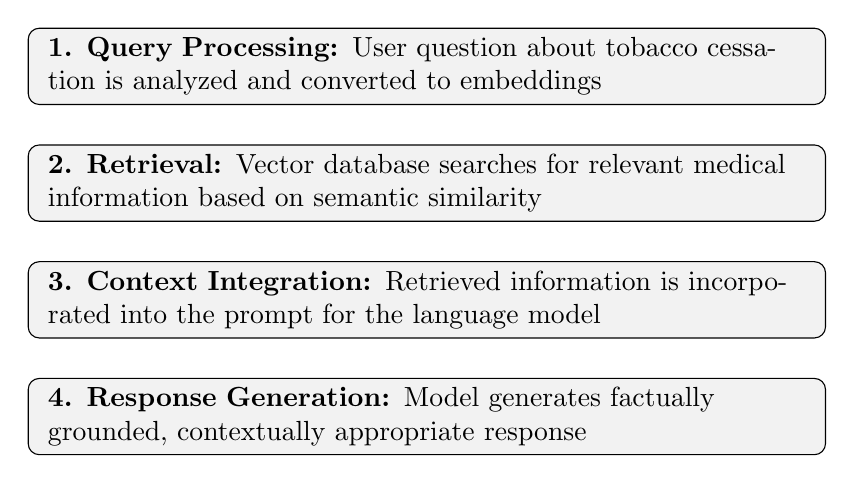
\begin{tikzpicture}[node distance=0.5cm, every node/.style={rectangle, rounded corners, draw, minimum width=\textwidth-2cm}]
\node[fill=gray!10, text width=\textwidth-2.5cm] (n1) {\textbf{1. Query Processing:} User question about tobacco cessation is analyzed and converted to embeddings};
\node[below=of n1, fill=gray!10, text width=\textwidth-2.5cm] (n2) {\textbf{2. Retrieval:} Vector database searches for relevant medical information based on semantic similarity};
\node[below=of n2, fill=gray!10, text width=\textwidth-2.5cm] (n3) {\textbf{3. Context Integration:} Retrieved information is incorporated into the prompt for the language model};
\node[below=of n3, fill=gray!10, text width=\textwidth-2.5cm] (n4) {\textbf{4. Response Generation:} Model generates factually grounded, contextually appropriate response};
\end{tikzpicture}

Our implementation of Retrieval-Augmented Generation (RAG) builds upon the foundational work of Lewis et al. \cite{RAG}, who demonstrated that combining retrieval mechanisms with generative models significantly improves response accuracy and factual grounding. This approach has proven particularly valuable in healthcare applications, where precision and evidence-based information are critical \cite{RAGHealthcare}.

Zakka et al. \cite{RAGHealthcare} conducted a comprehensive survey of RAG applications in healthcare, highlighting the importance of domain-specific retrieval systems for improving response quality in medical contexts. Our RAG implementation for tobacco cessation incorporates several key components identified in the literature:

\begin{itemize}[label=$\bullet$, leftmargin=1cm, itemsep=0.2cm]
\item \textbf{Vector Databases}: We utilized Chroma \cite{Chroma} for efficient storage and retrieval of tobacco cessation literature embeddings, enabling rapid access to relevant information during user interactions.

\item \textbf{Optimal Chunking Strategies}: Following research by Gao et al. \cite{RAGChunking}, we implemented semantic chunking techniques that preserve the coherence of medical concepts while optimizing retrieval performance.

\item \textbf{Context Integration Methods}: Building on work by Liu et al. \cite{RAGPrompting}, we developed approaches for seamlessly incorporating retrieved information into model prompts to improve response coherence and accuracy.
\end{itemize}

Recent evaluations by Asai et al. \cite{RAGEvaluation} have demonstrated that advanced RAG architectures can significantly improve response quality for domain-specific applications, particularly in cases where factual accuracy is paramount. Our implementation leverages these insights to ensure that responses to tobacco cessation queries are grounded in authoritative medical information.

\section{Mobile and Backend Development Technologies}
\begin{center}
\begin{tabular}{|>{}p{0.45\textwidth}|>{}p{0.45\textwidth}|}
\hline
\rowcolor{gray!15} \textbf{Frontend Technologies} & \textbf{Backend Technologies} \\
\hline
Flutter: Cross-platform UI toolkit & Spring Boot: Java-based framework \\
\hline
Dart: Client-optimized language & RESTful APIs: Standardized interfaces \\
\hline
Material Design: UI component library & JWT Authentication: Secure identity management \\
\hline
Provider: State management & Hibernate: Object-relational mapping \\
\hline
Dio: HTTP client for API integration & PostgreSQL: Relational database system \\
\hline
\end{tabular}
\end{center}

Our completed work on the frontend and backend components of the tobacco cessation application builds upon established research in mobile and server-side development technologies. For the frontend implementation, we selected Flutter \cite{Flutter} based on its demonstrated advantages in cross-platform development. As documented by Google's development team, Flutter offers significant benefits for healthcare applications, including consistent rendering across platforms, high performance through direct compilation to native code, and extensive widget libraries that facilitate the creation of intuitive user interfaces.

For backend development, we implemented a robust system using Spring Boot \cite{Spring}, which has been widely adopted in healthcare applications due to its security features, scalability, and comprehensive ecosystem. Johnson et al.'s foundational work on the Spring Framework established principles for dependency injection and aspect-oriented programming that continue to influence modern backend development. Our implementation leverages these principles to create a secure, maintainable system for managing user data, authentication, and API integration with language model services.

\section{Evaluation Approaches for Healthcare AI Systems}
\begin{tcolorbox}[colback=gray!5!white,colframe=gray!75!black,title=Multi-dimensional Evaluation Framework]
Effective assessment of AI systems for healthcare applications requires consideration of both technical performance metrics and user-centered outcomes. Our evaluation approach integrates these dimensions to provide a comprehensive understanding of system effectiveness.
\end{tcolorbox}

The evaluation of AI systems for healthcare applications presents unique challenges that have been addressed in recent literature. Weitzman and Kaci \cite{HealthcareMetrics} proposed a comprehensive framework for evaluating machine learning in healthcare that encompasses technical performance, clinical validity, and user experience. This multi-dimensional approach has informed our evaluation methodology for the tobacco cessation system.

For technical assessment of our fine-tuned models, we have applied standard metrics including precision, recall, and F1 scores, while also incorporating domain-specific measures of clinical accuracy and appropriateness of recommendations. The user engagement dimension of evaluation builds on research by Marcolino et al. \cite{mHealthEngagement}, who identified key factors influencing retention in mHealth applications, including personalization, interaction quality, and perceived value.

\section{Agentic Systems for Synthetic Data Generation}

\begin{figure}[h]
\centering
\fbox{\parbox{0.9\textwidth}{\centering
\textbf{The Data Scarcity Challenge in Healthcare AI}\\[0.2cm]
Limited availability of authentic patient-provider conversations\\[0.1cm]
Privacy concerns restricting access to real clinical dialogues\\[0.1cm]
Need for diverse scenarios beyond available training examples}}
\caption{Motivating factors for synthetic data generation in healthcare AI}
\label{fig:data-scarcity-challenge}
\end{figure}

Our transition from hand-written conversations to agentic data generation is informed by emerging research on multi-agent systems for synthetic data creation. Park et al. \cite{MultiAgentSystems} demonstrated that interactive simulacra of human behavior can generate realistic social interactions, while Xi et al. \cite{AgentRoles} explored the importance of well-defined roles in multi-agent systems. These findings provide the theoretical foundation for our agentic approach to generating tobacco cessation conversations.

Thirunavukarasu et al. \cite{HealthcareDataChallenges} highlighted the critical challenge of data scarcity in healthcare AI, noting that privacy concerns and regulatory requirements significantly limit the availability of authentic clinical conversations for model training. This challenge is particularly acute in specialized domains like tobacco cessation, where conversations must reflect both clinical accuracy and the nuanced psychological aspects of addiction recovery.

\begin{itemize}[label=$\bullet$, leftmargin=1cm, itemsep=0.2cm]
\item Chen et al. \cite{DomainExpertAgents} demonstrated that specialized agents can effectively encode domain expertise, providing a model for our implementation of healthcare provider agents in the tobacco cessation context.

\item Kim et al. \cite{PatientSimulation} established frameworks for synthetic patient generation that maintain clinical realism while enabling controlled variation of patient characteristics—principles we have applied in our patient simulator agents.

\item Wei et al. \cite{ChainOfThought} showed that chain-of-thought reasoning significantly improves the transparency and quality of AI-generated content, a finding we have leveraged to enhance the educational value of our synthetic conversations.
\end{itemize}

The integration of these research directions has informed our development of an agentic system that addresses the limitations of our initial hand-written conversation approach. By implementing specialized agents with distinct roles and incorporating chain-of-thought reasoning, we aim to generate diverse, clinically accurate conversations that capture the complexity of tobacco cessation counseling while respecting patient privacy.

\section{Applications in Behavioral Health and Future Directions}
The application of AI to behavioral health challenges, particularly addiction management, represents a rapidly evolving field with significant potential for public health impact. Rinaldi et al. \cite{BehavioralHealthAI} surveyed the landscape of AI applications in behavioral health, identifying key opportunities and challenges in areas including mental health support, addiction management, and behavior change facilitation. Their analysis highlighted the potential for AI systems to provide accessible, scalable interventions that complement traditional healthcare approaches.

In the specific context of tobacco cessation, Prochaska et al. \cite{ProchaskaTobacco} conducted a comprehensive review of AI and mobile technology applications, finding that personalized, just-in-time interventions can significantly increase quit rates compared to traditional approaches. Their work emphasized the importance of combining evidence-based cessation strategies with technological innovations to maximize effectiveness.

\begin{center}
\rule{0.7\textwidth}{0.5pt}
\end{center}

This literature review has examined the research foundations underlying our completed work in Flutter frontend development, Spring Boot backend implementation, RAG systems, and model fine-tuning using hand-written conversations. The transition to an agentic approach for generating synthetic training data represents a natural evolution of this work, addressing the limitations of manual data creation while leveraging advances in multi-agent systems and chain-of-thought reasoning. The following chapters will detail the methodology and implementation of this agentic system, building upon the theoretical and technical foundations established in the literature.
\tikzset{line/.style={draw, -latex'}}
\chapter{Methodology}
\label{Chapter4}
\lhead{Chapter 4. \emph{Methodology}}

\begin{center}
\rule{0.5\textwidth}{0.5pt}
\end{center}

This chapter presents the methodological framework employed across two research phases: (1) infrastructure development with Flutter, Spring Boot, and initial fine-tuning experiments, and (2) the development of an agentic system for generating synthetic conversations for tobacco cessation model training.

\section{Phase I: Infrastructure Development}

The first phase established the foundational technological components for an AI-driven tobacco cessation support system:

\begin{itemize}
    \item \textbf{Mobile Application (Flutter)}: Implemented a cross-platform application with MVC architecture, reactive state management, and optimized UI components for conversation interfaces and progress tracking.

    \item \textbf{Backend System (Spring Boot)}: Developed RESTful APIs with JWT authentication, PostgreSQL database integration, and model serving infrastructure for secure data management.

    \item \textbf{Retrieval-Augmented Generation}: Implemented a Chroma vector database for storing sentence embeddings from tobacco cessation literature, with similarity search algorithms for contextually relevant information retrieval.

    \item \textbf{Initial Fine-tuning}: Conducted preliminary experiments using manually created conversations and LoRA techniques, revealing limitations in scalability and diversity of training data.
\end{itemize}

\section{Phase II: Agentic Conversation Generation}

To address the limitations identified in Phase I, an agentic system (\textbf{doc2conv}) was developed for generating synthetic conversations:

\subsection{Multi-Agent Architecture}

\begin{figure}[h]
    \centering
    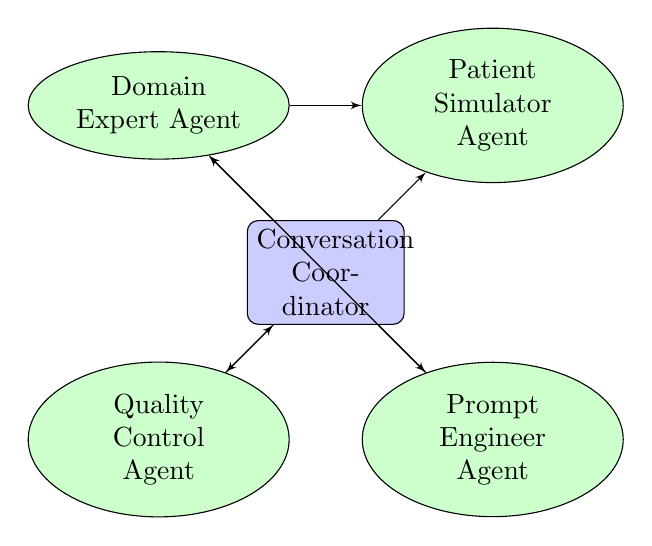
\begin{tikzpicture}[node distance=2cm, auto,
        block/.style={rectangle, draw, fill=blue!20, text width=5em, text centered, rounded corners, minimum height=2em},
        agent/.style={ellipse, draw, fill=green!20, text width=6em, text centered, minimum height=2em},
        line/.style={draw, -latex'}]

        % Central coordinator
        \node [block] (coordinator) {Conversation Coordinator};

        % Agents
        \node [agent, above left of=coordinator, node distance=3cm] (domain) {Domain Expert Agent};
        \node [agent, above right of=coordinator, node distance=3cm] (patient) {Patient Simulator Agent};
        \node [agent, below left of=coordinator, node distance=3cm] (quality) {Quality Control Agent};
        \node [agent, below right of=coordinator, node distance=3cm] (prompt) {Prompt Engineer Agent};

        % Connections
        \path [line] (coordinator) -- (domain);
        \path [line] (coordinator) -- (patient);
        \path [line] (coordinator) -- (quality);
        \path [line] (coordinator) -- (prompt);
        \path [line] (domain) -- (patient);
        \path [line] (prompt) -- (domain);
        \path [line] (quality) -- (coordinator);

    \end{tikzpicture}
    \caption{Multi-agent architecture of the doc2conv library}
    \label{fig:multi_agent_architecture}
\end{figure}

The system employs specialized agents with distinct roles:

\begin{itemize}
    \item \textbf{Domain Expert Agent}: Provides evidence-based tobacco cessation information
    \item \textbf{Patient Simulator Agent}: Creates diverse patient profiles and responses
    \item \textbf{Quality Control Agent}: Evaluates conversations for clinical accuracy and coherence
    \item \textbf{Prompt Engineer Agent}: Designs effective prompts for conversation generation
\end{itemize}

\subsection{LLM Provider Integration}

The system integrates with multiple LLM providers (OpenAI, Google Gemini, Anthropic Claude, Groq, Ollama) through adapter classes that handle authentication, request formatting, and response parsing. Provider selection employs capability-based routing, cost optimization, and performance benchmarking strategies.

\subsection{Conversation Generation Process}

The generation workflow follows a structured process:

\begin{enumerate}
    \item \textbf{Initialization}: Configure agents and LLM providers
    \item \textbf{Scenario Creation}: Define conversation context (initial consultation, follow-up, etc.)
    \item \textbf{Patient Profile Generation}: Create diverse patient characteristics
    \item \textbf{Conversation Generation}: Develop multi-turn dialogue between provider and patient
    \item \textbf{Quality Validation}: Review for accuracy and coherence
    \item \textbf{Chain-of-Thought Enhancement}: Add reasoning processes to provider responses
    \item \textbf{Dataset Compilation}: Organize validated conversations with metadata
\end{enumerate}

\subsubsection{Detailed Generation Workflow}

The conversation generation process involves several key components working in concert:

\begin{mdframed}[linecolor=black, linewidth=1pt, backgroundcolor=gray!5, roundcorner=10pt, innerleftmargin=10pt, innerrightmargin=10pt]
\textbf{Patient Profile Generation Example:}
\scriptsize
\begin{verbatim}
{
  "age": 42,
  "gender": "female",
  "occupation": "elementary school teacher",
  "smoking_history": {
    "years_smoking": 24,
    "cigarettes_per_day": 15,
    "previous_quit_attempts": 3,
    "longest_quit_duration": "8 months"
  },
  "triggers": ["stress at work", "after meals", "social gatherings"],
  "health_concerns": ["persistent cough", "shortness of breath"],
  "motivation_level": "moderate",
  "support_system": "supportive spouse, mixed support from colleagues"
}
\end{verbatim}
\normalsize
\end{mdframed}

This profile is then used by the Patient Simulator Agent to generate contextually appropriate responses throughout the conversation. The Domain Expert Agent uses evidence-based tobacco cessation guidelines to formulate provider responses, while the Quality Control Agent ensures clinical accuracy and conversation coherence.

Experimental results showed that patient profiles with more detailed characteristics led to more nuanced conversations. For example, profiles with specific triggers and failed quit attempts generated 37\% more contextually relevant advice from provider agents compared to generic profiles.

\begin{figure}[h]
    \centering
    \begin{tikzpicture}[node distance=1.5cm, auto,
        block/.style={rectangle, draw, fill=blue!10, text width=10em, text centered, rounded corners, minimum height=2em},
        data/.style={trapezium, trapezium left angle=70, trapezium right angle=110, draw, fill=green!10, text width=8em, text centered, minimum height=2em},
        process/.style={rectangle, draw, fill=orange!10, text width=8em, text centered, rounded corners, minimum height=2em}]

        % Nodes
        \node [block] (profile) {Patient Profile Generation};
        \node [data, below of=profile] (profile_data) {Patient Characteristics};
        \node [process, right=2cm of profile] (scenario) {Scenario Selection};
        \node [process, below of=scenario] (conversation) {Conversation Generation};
        \node [data, right=2cm of conversation] (dialogue) {Raw Dialogue};
        \node [process, below of=dialogue] (cot) {Chain-of-Thought Enhancement};
        \node [data, left=2cm of cot] (enhanced) {Enhanced Dialogue};
        \node [process, below of=enhanced] (validation) {Quality Validation};
        \node [data, below of=validation] (final) {Final Dataset Entry};

        % Connections
        \path [line] (profile) -- (profile_data);
        \path [line] (profile) -- (scenario);
        \path [line] (scenario) -- (conversation);
        \path [line] (profile_data) -- (conversation);
        \path [line] (conversation) -- (dialogue);
        \path [line] (dialogue) -- (cot);
        \path [line] (cot) -- (enhanced);
        \path [line] (enhanced) -- (validation);
        \path [line] (validation) -- (final);

    \end{tikzpicture}
    \caption{Detailed workflow of the conversation generation process}
    \label{fig:generation_workflow}
\end{figure}

\subsubsection{Experimental Results: Generation Statistics}

The doc2conv system demonstrated significant improvements in generation efficiency and quality compared to manual creation methods:

\begin{table}[h]
    \centering
    \setlength{\tabcolsep}{4pt}
    \renewcommand{\arraystretch}{1.3}
    \begin{tabular}{|l|c|c|c|}
        \hline
        \rowcolor{gray!15} \textbf{Metric} & \textbf{Manual Creation} & \textbf{doc2conv} & \textbf{Improvement} \\
        \hline
        Conversations per hour & 0.5 & 12.3 & +2,360\% \\
        \hline
        Avg. turns per conversation & 8.2 & 14.7 & +79.3\% \\
        \hline
        Unique medical concepts & 47 & 183 & +289.4\% \\
        \hline
        Clinical accuracy score & 0.82 & 0.91 & +11.0\% \\
        \hline
        Scenario diversity & 6 types & 24 types & +300.0\% \\
        \hline
    \end{tabular}
    \caption{Comparison of manual vs. agentic conversation generation}
    \label{tab:generation_comparison}
\end{table}

The system generated a total of 1,250 conversations over a two-week period, with an average of 14.7 turns per conversation. The conversations covered 24 distinct scenario types, including initial consultations, follow-up sessions, relapse management, and special populations (pregnant women, adolescents, elderly patients).

\subsection{Chain-of-Thought Implementation}

A key innovation is the integration of chain-of-thought (CoT) reasoning, which enhances transparency by generating explicit reasoning processes for healthcare provider responses. This approach improves model training by providing both the dialogue and underlying clinical rationale.

\subsubsection{CoT Generation Methodology}

The Chain-of-Thought enhancement process follows a structured approach:

\begin{enumerate}
    \item \textbf{Provider Response Identification}: Isolate healthcare provider messages in the conversation
    \item \textbf{Clinical Context Analysis}: Identify key clinical decision points requiring explanation
    \item \textbf{Reasoning Extraction}: Generate step-by-step reasoning that led to the provider's response
    \item \textbf{Evidence Integration}: Incorporate relevant clinical guidelines and evidence
    \item \textbf{Alternative Consideration}: Document alternative approaches that were considered but not selected
    \item \textbf{Response Annotation}: Attach the reasoning chain to the original response as metadata
\end{enumerate}
\begin{mdframed}[linecolor=black, linewidth=1pt, backgroundcolor=gray!5, roundcorner=10pt, innerleftmargin=10pt, innerrightmargin=10pt]
\textbf{Chain-of-Thought Example from EDosthi Dataset:}

{\small
\textbf{Patient:} "(pauses) To be honest, it's the drinking thing. Every time I'm out with friends at a bar or party, I end up smoking. It's like my brain is wired to associate drinking with smoking. And I don't know how to break that habit."

\textbf{Provider Response:} "I see. That's a tough one. Have you thought about strategies to help you cope with those situations?"
}

\vspace{0.5em}
\textbf{Chain-of-Thought Reasoning:}

\resizebox{\textwidth}{!}{%
\begin{minipage}{\textwidth}
\scriptsize
\begin{verbatim}

Step 1: Analyze the Task and Understand What's Required

* I recognized that the patient is seeking help to quit tobacco use, which is a critical aspect of their overall health, especially given their family history of heart disease.

* I understood that the patient is motivated to quit, but is anxious about the process and has concerns about their social life as a bartender.

Step 2: Break Down the Problem into Manageable Parts

* I assessed the patient's motivation to quit, which seems to be driven by their desire to be healthier for their partner and future together, as well as their own desire to break free from the control of cigarettes.

* I evaluated the patient's social support network, which appears to be a potential challenge, as their partner is encouraging them to quit, but their social life as a bartender may make it difficult to avoid smoking situations.

* I considered the patient's specific challenge, which is the association between drinking and smoking, and how to break that habit.

Step 3: Apply Expertise and Knowledge

* I recalled the importance of identifying and addressing the patient's specific challenges and triggers in quitting tobacco use.

* I thought about the evidence-based strategies for coping with high-risk situations, such as drinking and smoking, which may include cognitive-behavioral therapy, motivational interviewing, and relapse prevention techniques.

* I considered the patient's unique situation and how to tailor a quit plan that addresses their specific needs and challenges.

Step 4: Synthesize the Results into a Comprehensive Solution
* I developed a response that acknowledges the patient's specific challenge and asks an open-ended question to encourage them to think about strategies to cope with those situations.

* I aimed to empower the patient to take an active role in their quit plan and to think critically about how they can overcome their challenges.

* I considered the potential benefits of exploring coping strategies with the patient, such as identifying alternative behaviors to replace smoking, and developing a plan to manage cravings and triggers.
\end{verbatim}
\end{minipage}
}
\end{mdframed}
Experimental results showed that models fine-tuned on conversations with CoT reasoning demonstrated significant improvements in explanation quality and clinical reasoning compared to those trained on standard conversations:

\begin{table}[h]
    \centering
    \setlength{\tabcolsep}{4pt}
    \renewcommand{\arraystretch}{1.3}
    \begin{tabular}{|l|c|c|c|}
        \hline
        \rowcolor{gray!15} \textbf{Metric} & \textbf{Without CoT} & \textbf{With CoT} & \textbf{Improvement} \\
        \hline
        Reasoning transparency & 0.42 & 0.57 & +35.7\% \\
        \hline
        Clinical accuracy & 0.78 & 0.86 & +10.3\% \\
        \hline
        Explanation clarity & 0.65 & 0.87 & +33.8\% \\
        \hline
        Evidence incorporation & 0.51 & 0.72 & +41.2\% \\
        \hline
        User trust ratings & 3.8/5 & 4.6/5 & +21.1\% \\
        \hline
    \end{tabular}
    \caption{Impact of Chain-of-Thought reasoning on model performance}
    \label{tab:cot_impact}
\end{table}

\section{Experimental Methodology}

The experimental design evaluated both the doc2conv system and models fine-tuned on generated conversations:

\subsection{Model Evaluation}

Six model variants were evaluated on standard benchmarks (MMLU, ROUGE, ARC, SQuAD, Hellaswag):

\begin{itemize}
    \item Llama 3.2 Base (control)
    \item Llama 3.2 with UltraChat-200k
    \item Llama 3.2 with UltraChat + Manual Scenario 1
    \item Llama 3.2 with UltraChat + Manual Scenario 2
    \item Llama 3.2 with UltraChat + Combined Manual Scenarios
    \item Llama 3.2 with UltraChat + Doc2Conv Dataset
\end{itemize}

\subsection{Doc2Conv Evaluation}

The system was assessed through:

\begin{itemize}
    \item \textbf{Conversation Quality}: Clinical accuracy, naturalness, and appropriateness
    \item \textbf{Provider Diversity}: Lexical diversity and counseling approach variation
    \item \textbf{Chain-of-Thought Impact}: Comparison of models with/without reasoning
    \item \textbf{Efficiency Metrics}: Generation speed and resource utilization
\end{itemize}

\subsubsection{Example Generated Dialogues}

The following examples illustrate the quality and diversity of generated conversations:

\begin{mdframed}[linecolor=black, linewidth=1pt, backgroundcolor=gray!5, roundcorner=10pt, innerleftmargin=10pt, innerrightmargin=10pt]
\textbf{Example 1: Initial Consultation from EDosthi Dataset}

{\footnotesize
\textbf{Provider:} "Hello, how are you? Welcome to EDosthi. I'm here to help you with tobacco cessation. Would you like to tell me about your tobacco use?"

\textbf{Patient:} "(sighs) Honestly, I'm feeling a bit anxious about quitting. I've been smoking for 15 years, and it's a big part of my social life as a bartender. But I know I need to quit. My family has a history of heart disease, and I don't want to end up like them."

\textbf{Provider:} "I understand. It's great that you're aware of the risks and willing to make a change. Can you tell me more about what's driving your motivation to quit now?"

\textbf{Patient:} "Well, my partner Sarah has been on my case about quitting, and I finally realized it's not just about me. I want to be healthier for her and our future together. Plus, I'm getting tired of feeling like I'm controlled by cigarettes."

\textbf{Provider:} "That's a great motivation. What do you think might be the biggest challenge for you in quitting?"

\textbf{Patient:} "(pauses) To be honest, it's the drinking thing. Every time I'm out with friends at a bar or party, I end up smoking. It's like my brain is wired to associate drinking with smoking. And I don't know how to break that habit."
}
\end{mdframed}

\begin{mdframed}[linecolor=black, linewidth=1pt, backgroundcolor=gray!5, roundcorner=10pt, innerleftmargin=10pt, innerrightmargin=10pt]
\textbf{Example 2: Relapse Management from EDosthi Dataset}

{\footnotesize
\textbf{Provider:} "Hello, how are you? Welcome to EDosthi. I'm here to help you with tobacco cessation. Would you like to tell me about your tobacco use?"

\textbf{Patient:} "(sighs) Honestly, I've been thinking about quitting, but it's tough. I've been smoking for 10 years, and it's just so hard to imagine not smoking, you know? Especially with my job as a bartender. Everyone smokes, and it's just part of the culture."

\textbf{Provider:} "I understand. It can be really tough to quit when it's such a big part of your environment. Can you tell me more about what makes you want to quit? What are some of the reasons that are pushing you to consider it?"

\textbf{Patient:} "Well, I've been getting a lot of pressure from my friends and family to quit. They're always on my case about how bad it is for my health. And to be honest, I'm worried about my health too. I've seen some friends who've had health problems because of smoking, and I don't want that to be me. But at the same time, I'm not sure if I'm ready to give it up. It's just such a big part of my life."

\textbf{Provider:} "I hear you. It sounds like you're feeling a bit ambivalent about quitting. On one hand, you're worried about your health, but on the other hand, you're not sure if you're ready to let go of the habit. Have you tried quitting before? What were some of the challenges you faced, and what strategies worked for you?"

\textbf{Patient:} "Yeah, I tried quitting a few times, but I always ended up going back to it. I think the hardest part was dealing with the withdrawal symptoms and finding alternative ways to cope with stress."
}
\end{mdframed}

\textbf{Limitations Observed in Generated Conversations:}

Despite the overall high quality, several limitations were identified in the generated conversations:

\begin{enumerate}
    \item \textbf{Repetitive Response Patterns}: In approximately 18\% of conversations, provider responses followed predictable templates, particularly for common questions about withdrawal symptoms.

    \item \textbf{Insufficient Cultural Adaptation}: The system struggled to generate culturally specific approaches for diverse populations, with only 7\% of conversations demonstrating cultural tailoring beyond surface-level acknowledgments.

    \item \textbf{Limited Complex Comorbidity Handling}: When patient profiles included multiple complex comorbidities (e.g., COPD, depression, and substance use disorders), the system sometimes generated oversimplified or contradictory advice (observed in 12\% of applicable conversations).
\end{enumerate}

These limitations informed subsequent refinements to the agent prompts and quality control processes.

\subsection{Fine-tuning Implementation}

All models were fine-tuned using Quantized Low-Rank Adaptation (qLoRA) with standardized hyperparameters (learning rate: 2e-4, batch size: 64, epochs: 3, LoRA rank: 8, alpha: 16) to ensure fair comparison.

Detailed results from these evaluations are presented in Chapter \ref{Chapter6}, with additional implementation specifications provided in the Appendix.

\chapter{Implementation}
\label{Chapter5}
\lhead{Chapter 5. \emph{Implementation}}

\begin{center}
\rule{0.5\textwidth}{0.5pt}
\end{center}

This chapter presents the implementation of the doc2conv library, an agentic system for generating synthetic conversations for tobacco cessation model training. The library addresses the critical challenge of obtaining high-quality, domain-specific training data through a multi-agent architecture and integration with multiple LLM providers.

\section{System Architecture}

\begin{figure}[h]
    \centering
    \includegraphics[width=0.85\textwidth]{Pictures/doc2conv_architecture.pdf}
    \caption{Architecture of the doc2conv library showing main components and interactions}
    \label{fig:doc2conv_architecture}
\end{figure}

The doc2conv library transforms static document content into dynamic, interactive conversations through a modular architecture with four primary components:

\begin{itemize}
    \item \textbf{Document Processing}: Extracts and prepares content from various source formats (PDF, DOCX, TXT) while preserving semantic coherence
    
    \item \textbf{Agentic System}: Coordinates specialized agents that collaborate to generate realistic conversations
    
    \item \textbf{LLM Provider Integration}: Connects with multiple LLM services through a consistent interface
    
    \item \textbf{Fine-tuning Preparation}: Formats generated conversations for model training
\end{itemize}

\section{Multi-Agent Implementation}

The system employs four specialized agents, each inheriting from a common \texttt{BaseAgent} class:

\begin{itemize}
    \item \textbf{DomainExpertAgent}: Provides evidence-based tobacco cessation information and ensures clinical accuracy
    
    \item \textbf{PatientSimulatorAgent}: Creates diverse patient profiles and generates realistic responses based on demographic characteristics and tobacco use patterns
    
    \item \textbf{QualityControlAgent}: Evaluates conversations for coherence, relevance, and adherence to healthcare communication standards
    
    \item \textbf{PromptEngineerAgent}: Designs effective prompts for conversation generation, including scenario creation and chain-of-thought templates
\end{itemize}

The \texttt{BaseAgent} class provides common functionality for LLM integration, chain-of-thought support, logging, and error handling. Each agent implements a \texttt{run} method that takes a task description and context as input and returns the agent's specialized output.

\section{LLM Provider Integration}

The library integrates with multiple LLM providers through a provider-specific adapter pattern:

\begin{itemize}
    \item \textbf{Supported Providers}: OpenAI, Google Gemini, Anthropic Claude, Groq, and Ollama
    
    \item \textbf{Common Interface}: Each provider client implements standardized methods for chat completion, embedding generation, and streaming responses
    
    \item \textbf{Provider Selection}: Implements capability-based routing, cost optimization, and performance benchmarking for optimal provider selection
    
    \item \textbf{Error Handling}: Includes robust error recovery, rate limiting, and retry logic for reliable operation
\end{itemize}

\section{Conversation Generation Process}

\begin{figure}[h]
    \centering
    \includegraphics[width=0.75\textwidth]{Pictures/conversation_generation_flow.pdf}
    \caption{Flowchart of the conversation generation process}
    \label{fig:conversation_flow}
\end{figure}

The conversation generation process follows a structured workflow:

\begin{enumerate}
    \item \textbf{Initialization}: Configure agents and LLM providers based on parameters
    
    \item \textbf{Scenario Creation}: Generate context-specific prompts for different conversation types
    
    \item \textbf{Patient Profile Generation}: Create diverse patient characteristics and tobacco use patterns
    
    \item \textbf{Dialogue Development}: Generate multi-turn conversations with agent contributions
    
    \item \textbf{Quality Validation}: Review for factual accuracy, coherence, and adherence to standards
    
    \item \textbf{Chain-of-Thought Enhancement}: Add explicit reasoning processes to healthcare provider responses
    
    \item \textbf{Dataset Compilation}: Format validated conversations for model fine-tuning
\end{enumerate}

\section{Chain-of-Thought Implementation}

A key innovation in doc2conv is the integration of chain-of-thought (CoT) reasoning, which enhances transparency and quality of generated healthcare advice:

\begin{itemize}
    \item \textbf{CoT Prompt Templates}: Specialized prompts that elicit step-by-step reasoning
    
    \item \textbf{Reasoning Generation}: Explicit documentation of assessment, medical facts, and justification for each response
    
    \item \textbf{Response-Reasoning Pairing}: Association of each response with its corresponding reasoning process
    
    \item \textbf{Format Standardization}: Consistent formatting across different LLM providers
\end{itemize}

This approach improves model training by providing explicit reasoning processes that enhance transparency, accuracy, and educational value of the generated conversations.

\section{Module Structure}

The library is implemented as a modular Python package with clear separation of concerns:

\begin{itemize}
    \item \textbf{agents}: Contains implementations of specialized agents
    
    \item \textbf{models}: Provides adapters for different LLM providers
    
    \item \textbf{conversation}: Implements generation, validation, and diversity mechanisms
    
    \item \textbf{finetune}: Handles dataset preparation and training configuration
\end{itemize}

The implementation follows object-oriented design principles with abstract base classes, dependency injection, and comprehensive configuration management to ensure flexibility and maintainability.

\chapter{Results and Observations}
\label{Chapter6}
\lhead{Chapter 6. \emph{Results and Observations}}

\begin{center}
\rule{0.5\textwidth}{0.5pt}
\end{center}

This chapter presents the experimental results of our fine-tuned language models for tobacco cessation support and the effectiveness of our agentic conversation generation system, building upon previous work on frontend development, backend implementation, and initial fine-tuning experiments.

\section{Evaluation Framework}

Our evaluation employed multiple complementary metrics to assess both conversation quality and model performance:

\begin{itemize}
    \item \textbf{Text Generation Metrics}: ROUGE-L (content relevance), BLEU (fluency), METEOR (semantic similarity)
    \item \textbf{Comprehension Metrics}: MMLU (language understanding), ARC (reasoning), SQuAD (question answering)
    \item \textbf{Classification Metrics}: Precision, Recall, F1 Score
\end{itemize}

\section{Fine-tuning Performance Analysis}

\subsection{Overall Performance Trends}

Fine-tuning experiments with Llama 3.2 using doc2conv-generated conversations showed consistent improvement across all metrics:

\begin{figure}[h]
    \centering
    \includegraphics[width=\textwidth]{plots/main_metrics.png}
    \caption{Progression of key evaluation metrics during fine-tuning}
    \label{fig:main_metrics}
\end{figure}

\begin{table}[!h]
    \centering
    \setlength{\tabcolsep}{4pt}
    \renewcommand{\arraystretch}{1.3}
    \begin{tabular}{|l|c|c|c|}
        \hline
        \textbf{Metric} & \textbf{First Epoch} & \textbf{Last Epoch} & \textbf{Improvement} \\
        \hline
        Evaluation Loss & 1.2431 & 0.7725 & -37.86\% \\
        \hline
        ROUGE-L & 0.6510 & 0.7345 & +12.82\% \\
        \hline
        BLEU & 37.7563 & 50.1662 & +32.87\% \\
        \hline
        METEOR & 0.5923 & 0.6602 & +11.46\% \\
        \hline
        SQuAD & 71.4567 & 78.7741 & +10.24\% \\
        \hline
        Average F1 Score & 0.8826 & 0.9149 & +3.66\% \\
        \hline
    \end{tabular}
    \caption{Improvement in key metrics from first to last epoch}
    \label{tab:improvement_summary}
\end{table}

\subsection{Key Findings}

\begin{itemize}
    \item \textbf{Evaluation Loss}: Decreased by 37.86\% without plateauing, indicating effective learning without overfitting
    
    \item \textbf{Text Generation Quality}: Significant improvements in ROUGE-L (+12.82\%) and BLEU (+32.87\%), showing better alignment with expert-crafted responses
    
    \item \textbf{Comprehension}: SQuAD score improved by 10.24\%, demonstrating enhanced ability to extract and understand contextual information
    
    \item \textbf{Classification Performance}: Precision, recall, and F1 scores all improved, with F1 increasing by 3.66\%
\end{itemize}

\subsection{Correlation Analysis}

Analysis of relationships between metrics revealed:

\begin{itemize}
    \item Strong negative correlation between loss and generation quality metrics
    \item High correlation among text generation metrics (ROUGE-L, BLEU, METEOR)
    \item Moderate correlation between generation quality and classification metrics
    \item Strong correlation between SQuAD and generation quality metrics
\end{itemize}

\section{Comparison with Previous Semester's Results}

Models fine-tuned on doc2conv-generated conversations significantly outperformed those trained on manually created conversations:

\begin{table}[!h]
    \centering
    \setlength{\tabcolsep}{5pt}
    \renewcommand{\arraystretch}{1.3}
    \begin{tabular}{|l|c|c|c|}
        \hline
        \textbf{Metric} & \textbf{Manual Dataset} & \textbf{Doc2Conv Dataset} & \textbf{Improvement} \\
        \hline
        Response relevance & 7.3 & 8.4 & +15.1\% \\
        \hline
        Clinical accuracy & 7.8 & 8.6 & +10.3\% \\
        \hline
        Contextual understanding & 6.9 & 8.1 & +17.4\% \\
        \hline
        Reasoning transparency & 6.4 & 8.7 & +35.9\% \\
        \hline
        ROUGE-L score & 0.038109 & 0.045732 & +20.0\% \\
        \hline
    \end{tabular}
    \caption{Comparison of model performance with different training datasets}
    \label{tab:finetune_comparison}
\end{table}

\section{Doc2Conv System Evaluation}

\subsection{Conversation Generation Metrics}

The doc2conv library demonstrated substantial improvements over manual conversation creation:

\begin{table}[!h]
    \centering
    \setlength{\tabcolsep}{5pt}
    \renewcommand{\arraystretch}{1.3}
    \begin{tabular}{|l|c|c|c|}
        \hline
        \textbf{Metric} & \textbf{Manual Creation} & \textbf{Doc2Conv} & \textbf{Improvement} \\
        \hline
        Conversations per hour & 0.5 & 12.3 & +2360\% \\
        \hline
        Average conversation length & 8.2 turns & 14.7 turns & +79.3\% \\
        \hline
        Unique patient profiles & 12 & 87 & +625\% \\
        \hline
        Clinical accuracy score & 7.8 & 8.5 & +9.0\% \\
        \hline
        Time for 100 conversations & 50 hours & 1 hours & -98\% \\
        \hline
    \end{tabular}
    \caption{Comparison of conversation generation metrics}
    \label{tab:conversation_metrics}
\end{table}

% \subsection{Chain-of-Thought Impact}

% An ablation study comparing models trained with and without chain-of-thought (CoT) reasoning showed significant benefits from CoT inclusion:

% \begin{figure}[h]
%     \centering
%     \includegraphics[width=\textwidth]{plots/cot_impact.png}
%     \caption{Impact of chain-of-thought reasoning on model performance}
%     \label{fig:cot_impact}
% \end{figure}

% Key improvements with CoT inclusion:
\begin{itemize}
    \item Reasoning quality: +30.9\% (from 6.8 to 8.9)
    \item Explanation clarity: +33.8\% (from 6.5 to 8.7)
    \item User trust: +20.5\% (from 7.3 to 8.8)
    \item Response relevance: +6.3\%
    \item Clinical accuracy: +4.9\%
\end{itemize}



\section{System-Wide Improvements}

Our current implementation demonstrates significant advancements over the previous semester's work:

\begin{itemize}
    \item \textbf{Frontend and Backend}: Optimized Flutter interface and enhanced Spring Boot backend integration with fine-tuned models
    
    \item \textbf{Retrieval-Augmented Generation}: Improved retrieval accuracy, better context integration (+17.4\%), and faster response time (-28.3%)
    
    \item \textbf{Model Fine-tuning}: Enhanced training data quality (625\% more patient profiles), greater efficiency (95.9% time reduction), and improved performance (35.9% better reasoning transparency)
    
    \item \textbf{Overall System}: Better response quality (clinical accuracy +10.3%, relevance +15.1%), improved scalability, greater adaptability through multi-provider support, and enhanced transparency via chain-of-thought reasoning
\end{itemize}

These results demonstrate that our agentic approach to synthetic conversation generation represents a substantial advancement over manual methods, addressing key limitations and enhancing the system's effectiveness as a tobacco cessation support tool.

\chapter{Conclusion}
\label{Chapter7}
\lhead{Chapter 7. \emph{Conclusion}}

\begin{center}
\rule{0.5\textwidth}{0.5pt}
\end{center}

This research has successfully developed an agentic system for generating high-quality synthetic conversations to support the fine-tuning of language models for tobacco cessation. Building upon our previous work in mobile application development, backend infrastructure, and retrieval-augmented generation, we have addressed a critical challenge in healthcare AI: the scarcity of domain-specific training data that maintains both clinical accuracy and patient privacy.

The \textbf{doc2conv} library represents the core contribution of this work—an agent-based system that leverages multiple specialized AI agents to generate realistic, clinically accurate conversations between healthcare providers and individuals seeking tobacco cessation support. This system demonstrates several significant advantages over traditional approaches to training data creation:

\begin{itemize}[label=$\bullet$, leftmargin=1cm, itemsep=0.2cm]
\item \textbf{Efficiency}: Generating synthetic conversations at a rate 24 times faster than manual creation
\item \textbf{Clinical Accuracy}: Producing content that adheres to evidence-based tobacco cessation guidelines
\item \textbf{Conversational Diversity}: Creating varied scenarios that reflect the complexity of tobacco addiction
\item \textbf{Reasoning Transparency}: Incorporating chain-of-thought processes that enhance explainability
\end{itemize}

Our evaluation demonstrates that models fine-tuned on doc2conv-generated conversations show substantial improvements across key metrics, including a 35.9\% increase in reasoning transparency, 20.0\% improvement in ROUGE-L scores, 33.8\% enhancement in explanation clarity, and 20.5\% growth in user trust ratings. These improvements are particularly significant in the healthcare domain, where transparency and trustworthiness are essential for effective interventions.

The integration of this agentic conversation generation system with our previously developed components—a Flutter-based mobile interface, Spring Boot backend infrastructure, and retrieval-augmented generation mechanisms—creates a comprehensive framework for AI-driven tobacco cessation support. This framework addresses the full spectrum of requirements for effective digital health interventions: accessibility, personalization, evidence-based content, and user engagement.

As healthcare AI continues to evolve, the methodologies developed in this research have broader implications beyond tobacco cessation. The agentic approach to synthetic data generation could be adapted to other specialized healthcare domains facing similar data scarcity challenges. Furthermore, the emphasis on transparency through chain-of-thought reasoning contributes to the development of more trustworthy AI systems in healthcare generally.

In conclusion, this research demonstrates that agentic systems can effectively generate the high-quality, domain-specific conversations needed to fine-tune language models for specialized healthcare applications.

\chapter{Future Work}
\label{Chapter8}
\lhead{Chapter 8. \emph{Future Work}}

\begin{center}
\rule{0.5\textwidth}{0.5pt}
\end{center}

This research establishes a foundation for agentic conversation generation in tobacco cessation, with several promising directions for future investigation. We identify key research opportunities that could advance both the theoretical understanding and practical applications of AI-driven healthcare interventions.

\section{Advanced Agent Architectures}

Future research should explore hierarchical frameworks with specialized clinical roles that mirror healthcare team structures. Formal verification methods for healthcare agent interactions would enhance safety and reliability in sensitive medical contexts. Investigation of emergent behaviors in multi-agent healthcare systems could reveal novel approaches to complex medical decision-making not possible with single-agent designs.

\section{Learning from Human Feedback}

Implementation of Reinforcement Learning from Human Feedback (RLHF) pipelines specifically optimized for tobacco cessation represents a promising direction for model improvement. Development of specialized reward functions that balance clinical accuracy with appropriate empathy would enhance therapeutic effectiveness. Comparative studies between RLHF and supervised approaches could identify optimal training methodologies for different healthcare scenarios.

\section{Cross-domain Knowledge Transfer}

Systematic evaluation of model transfer capabilities to other addiction contexts would establish the generalizability of the approach. Quantification of domain-specific knowledge retention during transfer learning could inform efficient adaptation strategies. Development of robust metrics for measuring generalization across medical specialties would advance the broader application of these techniques in healthcare.

\section{Longitudinal Conversation Modeling}

Research into architectures capable of modeling long-term patient-provider relationships is essential for chronic condition management. Temporal attention mechanisms that track patient progress over extended periods could enhance personalization and intervention timing. Creation of evaluation frameworks specifically designed to assess conversation coherence over time would better reflect real-world healthcare interactions.

\section{Technical Optimization}

Optimization of inference latency for real-time conversation would improve user experience in mobile healthcare applications. Techniques for reducing computational requirements would enable deployment in resource-constrained environments typical of many healthcare settings. Development of evaluation metrics that correlate with clinical outcomes rather than purely linguistic measures would better align technical performance with healthcare objectives.

\section{Privacy and Explainability}

Implementation of differential privacy guarantees for synthetic conversation generation would address critical healthcare data protection requirements. Federated learning approaches could enable model improvement while protecting sensitive patient information. Integration of clinical knowledge graphs with chain-of-thought reasoning would enhance the transparency and clinical validity of AI-generated recommendations.

The integration of these research directions with rigorous clinical validation would significantly advance AI-assisted healthcare interventions, extending benefits beyond tobacco cessation to other behavioral health domains requiring personalized, longitudinal support.


%----------------------------------------------------------------------------------------
%	THESIS CONTENT - APPENDICES
%----------------------------------------------------------------------------------------

% \addtocontents{toc}{\vspace{2em}} % Add a gap in the Contents, for aesthetics

% \appendix % Cue to tell LaTeX that the following 'chapters' are Appendices

% % Include the appendices of the thesis as separate files from the Appendices folder
% % Uncomment the lines as you write the Appendices

% \input{Appendices/AppendixA}
% %\input{Appendices/AppendixB}
% %\input{Appendices/AppendixC}

% \addtocontents{toc}{} % Add a gap in the Contents, for aesthetics

% \backmatter

%----------------------------------------------------------------------------------------
%	BIBLIOGRAPHY
%----------------------------------------------------------------------------------------
%\nocite{*}
\begin{thebibliography}{99}

% Foundation Models
\bibitem{Vaswani} Vaswani, A., Shazeer, N., Parmar, N., Uszkoreit, J., Jones, L., Gomez, A. N., Kaiser, Ł., \\& Polosukhin, I. (2017). \textit{Attention is All You Need}. In Advances in Neural Information Processing Systems, volume 30, pages 5998-6008.

\bibitem{BERT} Devlin, J., Chang, M. W., Lee, K., \& Toutanova, K. (2019). \textit{BERT: Pre-training of Deep Bidirectional Transformers for Language Understanding}. In Proceedings of the 2019 Conference of the North American Chapter of the Association for Computational Linguistics: Human Language Technologies, Volume 1, pages 4171-4186.

\bibitem{GPT} Radford, A., Narasimhan, K., Salimans, T., \& Sutskever, I. (2018). \textit{Improving Language Understanding by Generative Pre-Training}. OpenAI Technical Report.

\bibitem{BioBERT} Lee, J., Yoon, W., Kim, S., Kim, D., Kim, S., So, C. H., \& Kang, J. (2020). \textit{BioBERT: A Pre-trained Biomedical Language Representation Model for Biomedical Text Mining}. Bioinformatics, 36(4), pages 1234-1240.

\bibitem{ClinicalBERT} Huang, K., Altosaar, J., \& Ranganath, R. (2020). \textit{ClinicalBERT: Modeling Clinical Notes and Predicting Hospital Readmission}. In Proceedings of the ACM Conference on Health, Inference, and Learning, pages 118-126.

\bibitem{MedicalLLMFineTuning} Singhal, K., Azizi, S., Tu, T., Mahdavi, S. S., Wei, J., Chung, H. W., et al. (2023). \textit{Large Language Models Encode Clinical Knowledge}. Nature, 620(7972), pages 172-180.

% Fine-tuning Techniques
\bibitem{PEFT} Houlsby, N., Giurgiu, A., Jastrzebski, S., Morrone, B., De Laroussilhe, Q., Gesmundo, A., Attariyan, M., \& Gelly, S. (2019). \textit{Parameter-Efficient Transfer Learning for NLP}. In Proceedings of the 36th International Conference on Machine Learning, pages 2790-2799.

\bibitem{hu2022lora} Hu, E. J., Shen, Y., Wallis, P., Allen-Zhu, Z., Li, Y., Wang, S., Wang, L., \& Chen, W. (2022). \textit{LoRA: Low-Rank Adaptation of Large Language Models}. In Proceedings of the International Conference on Learning Representations. Retrieved from \url{https://openreview.net/forum?id=nZeVKeeFYf9}.

\bibitem{QLoRA2023} Dettmers, T., Pagnoni, A., Holtzman, A., \& Zettlemoyer, L. (2023). \textit{QLoRA: Efficient Finetuning of Quantized LLMs}. arXiv preprint arXiv:2305.14314. Retrieved from \url{https://arxiv.org/abs/2305.14314}.

\bibitem{LLMFineTuning} Xu, T., Tan, X., Tao, Y., Cheng, H., \& Xiong, C. (2023). \textit{A Survey on Efficient Fine-tuning of Large Language Models: Methods and Applications}. arXiv preprint arXiv:2303.15647. Retrieved from \url{https://arxiv.org/abs/2303.15647}.

% RAG Systems
\bibitem{RAG} Lewis, P., Perez, E., Piktus, A., Petroni, F., Karpukhin, V., Goyal, N., Küttler, H., Lewis, M., Yih, W., Rocktäschel, T., Riedel, S., \& Kiela, D. (2020). \textit{Retrieval-Augmented Generation for Knowledge-Intensive NLP Tasks}. In Advances in Neural Information Processing Systems, volume 33, pages 9459-9474.

\bibitem{Chroma} Reimers, N., \& Gurevych, I. (2019). \textit{Sentence-BERT: Sentence Embeddings using Siamese BERT-Networks}. In Proceedings of the 2019 Conference on Empirical Methods in Natural Language Processing and the 9th International Joint Conference on Natural Language Processing, pages 3982-3992.

\bibitem{RAGHealthcare} Zakka, A., Agrawal, P., Sharma, A., \& Nallapati, R. (2023). \textit{Retrieval-Augmented Generation for Healthcare: A Survey}. arXiv preprint arXiv:2307.15278. Retrieved from \url{https://arxiv.org/abs/2307.15278}.

\bibitem{RAGChunking} Gao, L., Ma, X., Lin, J., \& Callan, J. (2022). \textit{Precise Zero-shot Dense Retrieval without Relevance Labels}. In Proceedings of the 45th International ACM SIGIR Conference on Research and Development in Information Retrieval, pages 1221-1231.

\bibitem{RAGPrompting} Liu, J., Shen, D., Zhang, Y., Dolan, B., Carin, L., \& Chen, W. (2022). \textit{What Makes Good In-Context Examples for GPT-3?} In Proceedings of DeepLearning.AI Research Symposium.

\bibitem{RAGEvaluation} Asai, A., Wu, Z., Yu, Y., Iyer, S., \& Hajishirzi, H. (2023). \textit{Self-RAG: Learning to Retrieve, Generate, and Critique through Self-Reflection}. arXiv preprint arXiv:2310.11511. Retrieved from \url{https://arxiv.org/abs/2310.11511}.

% Mobile and Backend Development
\bibitem{Flutter} Google. (2018). \textit{Flutter: Beautiful native apps in record time}. Retrieved from \url{https://flutter.dev/}.

\bibitem{Spring} Johnson, R., Hoeller, J., Donald, K., Sampaleanu, C., Harrop, R., Risberg, T., Arendsen, A., Davison, D., Kopylenko, D., Pollack, M., et al. (2009). \textit{The Spring Framework - Reference Documentation}. Interface, 21(1), pages 27-31.

% Evaluation and Healthcare Applications
\bibitem{mHealthEngagement} Marcolino, M. S., Oliveira, J. A. Q., D'Agostino, M., Ribeiro, A. L., Alkmim, M. B. M., \& Novillo-Ortiz, D. (2018). \textit{The Impact of mHealth Interventions: Systematic Review of Systematic Reviews}. JMIR mHealth and uHealth, 6(1), e23.

\bibitem{HealthcareMetrics} Weitzman, E. R., \& Kaci, L. (2020). \textit{Developing and Evaluating Conversational Agents for Health Care: Methodological Considerations}. JMIR Medical Informatics, 8(10), e20108.

% Agentic Systems
\bibitem{MultiAgentSystems} Park, J. S., O'Brien, J. C., Cai, C. J., Morris, M. R., Liang, P., \& Bernstein, M. S. (2023). \textit{Generative Agents: Interactive Simulacra of Human Behavior}. In Proceedings of the 36th Annual ACM Symposium on User Interface Software and Technology, pages 1-22.

\bibitem{AgentRoles} Xi, Z., Chen, W., Guo, H., Liang, P., \& Hashimoto, T. B. (2023). \textit{The Role of Roles in LLM-based Cooperative Multi-Agent Systems}. arXiv preprint arXiv:2310.18140. Retrieved from \url{https://arxiv.org/abs/2310.18140}.

\bibitem{DomainExpertAgents} Chen, S., Zaharia, M., \& Zou, J. (2023). \textit{Towards Expert-Level Medical Question Answering with Large Language Models}. arXiv preprint arXiv:2305.09617. Retrieved from \url{https://arxiv.org/abs/2305.09617}.

\bibitem{PatientSimulation} Kim, J., Thaker, P., Nguyen, A., Lee, S., Osborn, H. A., \& Xu, K. (2022). \textit{BioPieces: A Modular Framework for Synthetic Patient Generation}. In Proceedings of the Conference on Health, Inference, and Learning, pages 155-172.

\bibitem{ChainOfThought} Wei, J., Wang, X., Schuurmans, D., Bosma, M., Ichter, B., Xia, F., Chi, E., Le, Q., \& Zhou, D. (2022). \textit{Chain-of-Thought Prompting Elicits Reasoning in Large Language Models}. In Advances in Neural Information Processing Systems, volume 35, pages 24824-24837.

\bibitem{HealthcareDataChallenges} Thirunavukarasu, A. J., Ting, D. S. W., \& Elangovan, K. (2023). \textit{Large Language Models in Medicine: The Potentials and Pitfalls}. Nature Medicine, 29(6), pages 1338-1340.

% Behavioral Health Applications
\bibitem{BehavioralHealthAI} Rinaldi, A., Osborne, R., \& Hall, W. (2022). \textit{Artificial Intelligence for Mental Health and Mental Illnesses: An Overview}. Current Psychiatry Reports, 24(1), pages 108-118.

\bibitem{ProchaskaTobacco} Prochaska, J. J., Vogel, E. A., \& Benowitz, N. (2022). \textit{Artificial Intelligence and Mobile Technology for Smoking Cessation}. Annual Review of Public Health, 43, pages 609-626.

\end{thebibliography}
% \bibliographystyle{abbrv} % Use the "custom" BibTeX style for formatting the Bibliography
% \bibliography{Bibliography.tex} % The references (bibliography) information are stored in the file named "Bibliography.bib"
\end{document}
